\documentclass[11pt,a4paper]{article}
\usepackage[utf8]{inputenc}
\usepackage[german]{babel}
\usepackage{amsmath}
\usepackage{amsfonts}
\usepackage{subfig}
\usepackage{amssymb}
\usepackage{siunitx,physics}
\usepackage{mathtools}
\usepackage{graphicx}
%\usepackage{Here}
\usepackage[version=4]{mhchem}
\usepackage{url}
\usepackage{setspace}
\usepackage[left=2.5cm,right=2.5cm,top=2.5cm,bottom=2cm]{geometry}
[biblography=totocnumbered]
\usepackage{fancyhdr}
\usepackage{scrextend}
\usepackage{hyperref}
\pagenumbering{gobble}

\makeatletter
\newcommand\bigcdot{\mathpalette\bigcdot@{.5}}
\newcommand\bigcdot@[2]{\mathbin{\vcenter{\hbox{\scalebox{#2}{$\m@th#1\bullet$}}}}}
\makeatother

\makeatletter
%\renewcommand*\bib@heading{%
%  \subsection*{}%
%  \@mkboth{\refname}{\refname}}
%\makeatother
\numberwithin{equation}{section}
\numberwithin{figure}{section}

\renewcommand{\labelitemii}{\labelitemfont$\vartriangleright$}
\begin{document}
\noindent\textbf{8. Was ist ein Arrhenius-Diagramm und was kann man darin ablesen? }\\
\begin{addmargin}[25pt]{0pt}
Im Arrhenius-Diagramm (Abbildung \ref{fig:arrhenius}) wird der Diffusionskoeffizient logarithmisch gegen den Kehrwert der Temperatur aufgetragen. Daraus kann man dann die Aktivierungsenergie und den Faktor $D_0$ ablesen. Der Schnittpunkt mit der $D$-Achse ist dabei der Vorfaktor $D_0$ und die Aktivierungsenergie bestimmt man aus der Steigung der entstehenden Geraden $-\frac{Q_d}{R\cdot\ln{10}}$ der Faktor $\ln{10}$ kommt daher, dass man den dekadischen Logarithmus zum plotten verwendet.\\
\begin{figure}[h]
    \centering
    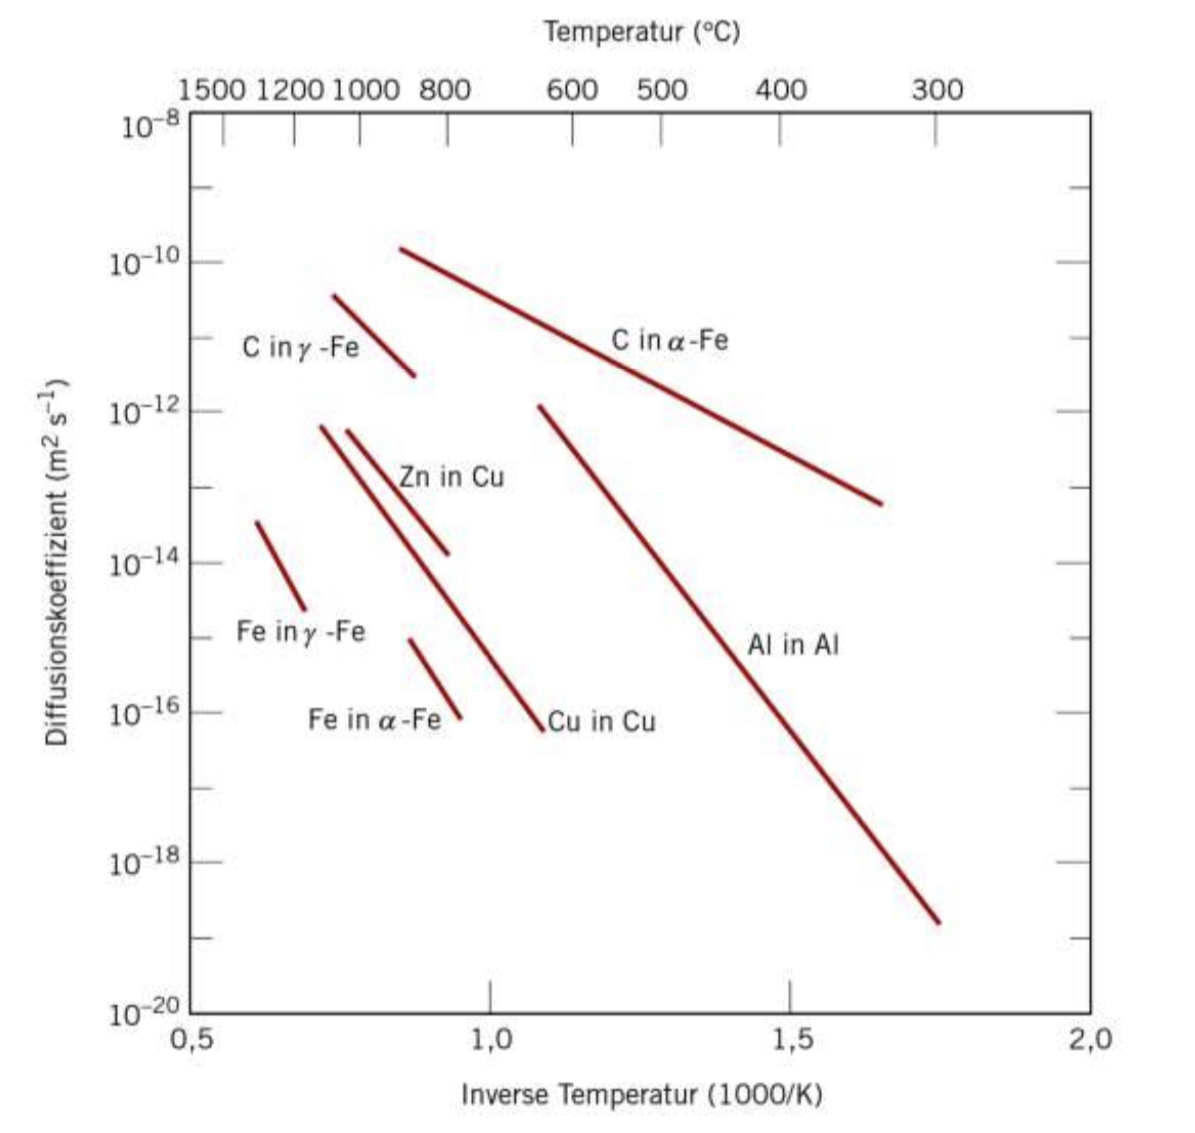
\includegraphics[width = 0.8\textwidth]{images/Materialwissenschaften/Arrhenius.jpeg}
    \caption{Arrhenius-Diagramm für verschiedene Stoffe}
    \label{fig:arrhenius}
\end{figure}
\end{addmargin} 
\end{document}
